\documentclass[]{article}
\usepackage{lmodern}
\usepackage{amssymb,amsmath}
\usepackage{ifxetex,ifluatex}
\usepackage{fixltx2e} % provides \textsubscript
\ifnum 0\ifxetex 1\fi\ifluatex 1\fi=0 % if pdftex
  \usepackage[T1]{fontenc}
  \usepackage[utf8]{inputenc}
\else % if luatex or xelatex
  \ifxetex
    \usepackage{mathspec}
  \else
    \usepackage{fontspec}
  \fi
  \defaultfontfeatures{Ligatures=TeX,Scale=MatchLowercase}
\fi
% use upquote if available, for straight quotes in verbatim environments
\IfFileExists{upquote.sty}{\usepackage{upquote}}{}
% use microtype if available
\IfFileExists{microtype.sty}{%
\usepackage{microtype}
\UseMicrotypeSet[protrusion]{basicmath} % disable protrusion for tt fonts
}{}
\usepackage[margin=1in]{geometry}
\usepackage{hyperref}
\hypersetup{unicode=true,
            pdftitle={Práctica 2 - Modelos Lineales 2},
            pdfauthor={Hernandez Bello Diana Patricia `20183808', Manrique Urbina Justo Andres `20091107', Moreano Roldan Juan Pablo `20184093', Parillo Apaza Jorge Hernan `19947810' , Urbano Burgos Alejandrina Margarita `20047278'},
            pdfborder={0 0 0},
            breaklinks=true}
\urlstyle{same}  % don't use monospace font for urls
\usepackage{color}
\usepackage{fancyvrb}
\newcommand{\VerbBar}{|}
\newcommand{\VERB}{\Verb[commandchars=\\\{\}]}
\DefineVerbatimEnvironment{Highlighting}{Verbatim}{commandchars=\\\{\}}
% Add ',fontsize=\small' for more characters per line
\usepackage{framed}
\definecolor{shadecolor}{RGB}{248,248,248}
\newenvironment{Shaded}{\begin{snugshade}}{\end{snugshade}}
\newcommand{\AlertTok}[1]{\textcolor[rgb]{0.94,0.16,0.16}{#1}}
\newcommand{\AnnotationTok}[1]{\textcolor[rgb]{0.56,0.35,0.01}{\textbf{\textit{#1}}}}
\newcommand{\AttributeTok}[1]{\textcolor[rgb]{0.77,0.63,0.00}{#1}}
\newcommand{\BaseNTok}[1]{\textcolor[rgb]{0.00,0.00,0.81}{#1}}
\newcommand{\BuiltInTok}[1]{#1}
\newcommand{\CharTok}[1]{\textcolor[rgb]{0.31,0.60,0.02}{#1}}
\newcommand{\CommentTok}[1]{\textcolor[rgb]{0.56,0.35,0.01}{\textit{#1}}}
\newcommand{\CommentVarTok}[1]{\textcolor[rgb]{0.56,0.35,0.01}{\textbf{\textit{#1}}}}
\newcommand{\ConstantTok}[1]{\textcolor[rgb]{0.00,0.00,0.00}{#1}}
\newcommand{\ControlFlowTok}[1]{\textcolor[rgb]{0.13,0.29,0.53}{\textbf{#1}}}
\newcommand{\DataTypeTok}[1]{\textcolor[rgb]{0.13,0.29,0.53}{#1}}
\newcommand{\DecValTok}[1]{\textcolor[rgb]{0.00,0.00,0.81}{#1}}
\newcommand{\DocumentationTok}[1]{\textcolor[rgb]{0.56,0.35,0.01}{\textbf{\textit{#1}}}}
\newcommand{\ErrorTok}[1]{\textcolor[rgb]{0.64,0.00,0.00}{\textbf{#1}}}
\newcommand{\ExtensionTok}[1]{#1}
\newcommand{\FloatTok}[1]{\textcolor[rgb]{0.00,0.00,0.81}{#1}}
\newcommand{\FunctionTok}[1]{\textcolor[rgb]{0.00,0.00,0.00}{#1}}
\newcommand{\ImportTok}[1]{#1}
\newcommand{\InformationTok}[1]{\textcolor[rgb]{0.56,0.35,0.01}{\textbf{\textit{#1}}}}
\newcommand{\KeywordTok}[1]{\textcolor[rgb]{0.13,0.29,0.53}{\textbf{#1}}}
\newcommand{\NormalTok}[1]{#1}
\newcommand{\OperatorTok}[1]{\textcolor[rgb]{0.81,0.36,0.00}{\textbf{#1}}}
\newcommand{\OtherTok}[1]{\textcolor[rgb]{0.56,0.35,0.01}{#1}}
\newcommand{\PreprocessorTok}[1]{\textcolor[rgb]{0.56,0.35,0.01}{\textit{#1}}}
\newcommand{\RegionMarkerTok}[1]{#1}
\newcommand{\SpecialCharTok}[1]{\textcolor[rgb]{0.00,0.00,0.00}{#1}}
\newcommand{\SpecialStringTok}[1]{\textcolor[rgb]{0.31,0.60,0.02}{#1}}
\newcommand{\StringTok}[1]{\textcolor[rgb]{0.31,0.60,0.02}{#1}}
\newcommand{\VariableTok}[1]{\textcolor[rgb]{0.00,0.00,0.00}{#1}}
\newcommand{\VerbatimStringTok}[1]{\textcolor[rgb]{0.31,0.60,0.02}{#1}}
\newcommand{\WarningTok}[1]{\textcolor[rgb]{0.56,0.35,0.01}{\textbf{\textit{#1}}}}
\usepackage{graphicx,grffile}
\makeatletter
\def\maxwidth{\ifdim\Gin@nat@width>\linewidth\linewidth\else\Gin@nat@width\fi}
\def\maxheight{\ifdim\Gin@nat@height>\textheight\textheight\else\Gin@nat@height\fi}
\makeatother
% Scale images if necessary, so that they will not overflow the page
% margins by default, and it is still possible to overwrite the defaults
% using explicit options in \includegraphics[width, height, ...]{}
\setkeys{Gin}{width=\maxwidth,height=\maxheight,keepaspectratio}
\IfFileExists{parskip.sty}{%
\usepackage{parskip}
}{% else
\setlength{\parindent}{0pt}
\setlength{\parskip}{6pt plus 2pt minus 1pt}
}
\setlength{\emergencystretch}{3em}  % prevent overfull lines
\providecommand{\tightlist}{%
  \setlength{\itemsep}{0pt}\setlength{\parskip}{0pt}}
\setcounter{secnumdepth}{0}
% Redefines (sub)paragraphs to behave more like sections
\ifx\paragraph\undefined\else
\let\oldparagraph\paragraph
\renewcommand{\paragraph}[1]{\oldparagraph{#1}\mbox{}}
\fi
\ifx\subparagraph\undefined\else
\let\oldsubparagraph\subparagraph
\renewcommand{\subparagraph}[1]{\oldsubparagraph{#1}\mbox{}}
\fi

%%% Use protect on footnotes to avoid problems with footnotes in titles
\let\rmarkdownfootnote\footnote%
\def\footnote{\protect\rmarkdownfootnote}

%%% Change title format to be more compact
\usepackage{titling}

% Create subtitle command for use in maketitle
\providecommand{\subtitle}[1]{
  \posttitle{
    \begin{center}\large#1\end{center}
    }
}

\setlength{\droptitle}{-2em}

  \title{Práctica 2 - Modelos Lineales 2}
    \pretitle{\vspace{\droptitle}\centering\huge}
  \posttitle{\par}
    \author{Hernandez Bello Diana Patricia `20183808', Manrique Urbina Justo Andres
`20091107', Moreano Roldan Juan Pablo `20184093', Parillo Apaza Jorge
Hernan `19947810' , Urbano Burgos Alejandrina Margarita `20047278'}
    \preauthor{\centering\large\emph}
  \postauthor{\par}
      \predate{\centering\large\emph}
  \postdate{\par}
    \date{10/26/2019}


\begin{document}
\maketitle

\hypertarget{pregunta-1}{%
\subsection{Pregunta 1}\label{pregunta-1}}

Sea \(Y\) una variable aleatoria discreta con distribución binomial
negativa \(\mu\) y parámetro de dispersión \(\phi\), cuya función de
distribución es dada por
\[ f{(y)}=\frac{\Gamma{(y+\phi)}}{\Gamma{(y+1)}\Gamma{(\phi)}}{(\frac{\mu}{\mu+\phi})}^{y}{(\frac{\phi}{\mu+\phi})}^{\phi}, y=0,1,2\ldots\]

Demuestre que pertenece a la familia exponencial, para \(\phi\)
conocido.

\textbf{Solución:} La función de probabilidad de \(Y\) se puede
reexpresar como:
\[ f{(y)}=\frac{\Gamma{(y+\phi)}}{\Gamma{(y+1)}\Gamma{(\phi)}}{(1-p)}^y+p^\phi.\]

Posteriormente, la función se puede expresar de la siguiente forma:

\[f{(y)}=\frac{\Gamma{(y+\phi)}}{\Gamma{(y+1)}\Gamma{(\phi)}} \exp(y \log(1-p) \phi \log(p).\]

En donde \(p=\frac{\phi}{\mu+\phi}\) y \(1-p=\frac{\mu}{\mu+\phi}\)

Se observa que pertenecería a la familia exponencial en tanto \(\phi\)
es conocido, pues:

\begin{itemize}
\tightlist
\item
  \(\theta=log(1-p)\)
\item
  \(b(\theta)=\phi\log(p)\) o, asimismo,
  \(b(\theta)=\phi\log(1-e^\theta)\)
\item
  \(c(y,\phi)\) es igual a la función gamma.
\item
  \(\phi=1\)
\end{itemize}

Demuestre que para \(\phi\) conocido, la distribución de \(Y\) pertenece
a la familia exponencial.

Encuentre la función de varianza y la función de enlace canónica.

\textbf{Solución:} La función de varianza se define como:
\[V(Y)=\frac{-1}{\phi}b^{''}(\theta)\]

Resolviendo, se tiene que:
\[ \frac{\partial^2}{\partial \theta^2} b(\theta)=\frac{\partial}{\partial \theta}(\frac{\phi e^\theta}{1-e^\theta})=\phi\frac{\partial}{\partial \theta}(\frac{ e^\theta}{1-e^\theta})=\phi \frac{e^\theta}{(1-e^\theta)^2}=\frac{\phi{(1-p)}}{p^2}\]

Reemplazando \(p\) y \(1-p\), se tiene que:

\[\frac{\frac{\phi \mu}{\mu+\phi}}{\frac{\phi^2}{(\mu+\phi)^2}}\]

Por lo tanto, la varianza es: \[\mu + \frac{\mu^2}{\phi}.\]

La función de enlace canónica se definiría de la siguiente forma:

\[\theta=\frac{\mu}{\phi+\mu}\]

\hypertarget{pregunta-2}{%
\subsection{Pregunta 2}\label{pregunta-2}}

\textbf{a)} Demuestre la matriz de información de Fisher para
\[\beta= (\beta_0,\beta_1)^T \]

En general, la matriz de información de Fisher está dada por:
\[I(\theta)= \phi\sum^n_{i=1}w_i x_i x_j\]

Esto, de forma matricial, se escribe de:

\[\phi X^TwX\]

Considerando que, para Poisson, el siguiente enlace:
\[\eta_i=\log(\mu_i)\]

y varianza \(V(\mu)=\mu\).

Asimismo, se tiene que:
\[w_i=\frac{(\frac{\partial}{\partial\eta_i})^2}{V_i}\]
\[w_i=\frac{(\frac{\partial\eta_i}{\partial})^{-2}}{V_i}\]

En dónde \(\frac{\partial \eta_i}{\partial \mu_i}=\frac{1}{\mu}\)

Por lo tanto, reemplazando en la ecuación anterior, se tiene que:
\[w_i=\frac{(\frac{1}{\mu})^{-2}}{V_i}\] \[w_i=\frac{\mu^2}{\mu}=\mu\]

Entonces se tiene que \(w_i=\mu_i\). Por lo tanto, la matriz de
información de Fisher es: \[\phi X^TwX\]

en dónde se tiene lo siguiente: \[\phi=1\]
\[w=diag(\mu_1,\mu_2,\ldots,\mu_n)\]

\textbf{b)} Encuentre una expresión de varianza de
\(\hat\beta_0 - \hat\beta_1\)

Se sabe que \(Var(\hat\beta)=(X^TwX)^{-1}\) para Poisson.

Para hallar \((X^TwX)\) (matriz de información de Fisher) se aplica:

\[H(\beta) =-\frac{\partial^2 l(\beta_0,\beta_1)}{\partial \beta  \partial\beta'}  = - \sum^n_{i=1}  \frac{\partial^2 l_i(\beta_0,\beta_1)}{\partial \beta  \partial\beta'}\]

Para el cálculo de
\(-\frac{\partial^2 l(\beta_0,\beta_1)}{\partial \beta \partial\beta'}\)
se consideran las siguientes notaciones :

\begin{itemize}
\tightlist
\item
  \[L_i(\beta_0,\beta_1) = u^{y_1}_i(exp(-\mu_i))\] como contribución de
  la observación i
\item
  \[L_i(\beta_0,\beta_1) = \prod^n_{i=1} L_i(\beta_0,\beta_1)\] como
  función de verosimilitud
\item
  \[l_i(\beta_0,\beta_1) = y_i log(\mu_i) - u_i = y_i(\beta_0+\beta_1 X_i) - exp(\beta_0+\beta_1 X_i)\]
  como logaritmo de la primera expresión
\end{itemize}

Luego

\[\frac{\partial^2 l_i(\beta_0,\beta_1)}{\partial \beta^2_0} = -exp(\beta_0+\beta_1 X_1) = - \mu_i\]

\[\frac{\partial^2 l_i(\beta_0,\beta_1)}{\partial \beta^2_1} = -exp(\beta_0+\beta_1) X^2_i = - \mu_i X^2_i\]

\[\frac{\partial^2 l_i(\beta_0,\beta_1)}{\partial \beta_0 \beta_1} = -exp(\beta_0+\beta_1) X_i = - \mu_i X_i\]

De lo anterior se tiene que \(H(\beta)\)

\[H(\beta) = \left(\begin{array}{cc} \sum^n_{i=1} \mu_i & \sum^n_{i=1} \mu_i x_i\\ \sum^n_{i=1} \mu_i x_i & \sum^n_{i=1} \mu_i x^2_i \end{array}\right)\]

Dado que \(H(\beta)=X^TwX\) y \(Var(\hat\beta)=(X^TwX)^{-1}\) se tiene
que :

\[Var(\hat\beta)=(H(\beta))^{-1} = \frac{1}{(\sum^n_i \mu_i)(\sum^n_i \mu_i x^2_i)- 
(\sum^n_i \mu_i X_i)^2} \left(\begin{array}{cc} \sum^n_i \mu_i  x^2_i& - \sum^n_i \mu_i x_i\\ - \sum^n_i \mu_i x_i & \sum^n_i \mu_i \end{array}\right)\]

Donde :
\[(\sum^n_{i=1} \mu_i)(\sum^n_{i=1} \mu_i x^2_i)-(\sum^n_{i=1} \mu_i X_i)^2 = Z\]

Se solicita :

\[Var(\hat\beta_0 - \hat\beta_1)= Var(\hat\beta_0) + Var(\hat\beta_1) - 2 Cov(\hat\beta_0,\hat\beta_1)\]

\[Z(\sum^n_{i=1} \mu_i X^2_i) + Z(\sum^n_{i=1} \mu_i) + 2 \sum^n_{i=1} \mu_i x_i \]

\hypertarget{pregunta-3}{%
\subsection{Pregunta 3}\label{pregunta-3}}

\begin{Shaded}
\begin{Highlighting}[]
\NormalTok{datos <{-}}\StringTok{ }\KeywordTok{read.csv}\NormalTok{(}\StringTok{"\textasciitilde{}/Documents/maestria{-}pucp/2019{-}2/modelos{-}lineales{-}2/clase{-}7/Preg3.csv"}\NormalTok{, }\DataTypeTok{sep=}\StringTok{","}\NormalTok{,}\DataTypeTok{fileEncoding =} \StringTok{"UTF{-}8"}\NormalTok{)}
\end{Highlighting}
\end{Shaded}

\begin{Shaded}
\begin{Highlighting}[]
\KeywordTok{library}\NormalTok{(glm2)}
\KeywordTok{library}\NormalTok{(faraway)}
\KeywordTok{library}\NormalTok{(car)}
\KeywordTok{library}\NormalTok{(spm)}
\KeywordTok{library}\NormalTok{(MASS)}
\KeywordTok{library}\NormalTok{(hnp)}
\KeywordTok{library}\NormalTok{(ggplot2)}
\end{Highlighting}
\end{Shaded}

En el archivo Preg3.csv se presentan los siguientes variables medidas
durante un año en una región :

\begin{itemize}
\item
  reclamos : números de reclamos en un seguro de autos para
  responsabilidad civil frente a terceros.
\item
  accidentes : números de accidetes en la región
\item
  poblacion : poblacion en la región
\end{itemize}

\textbf{a)} Estime un modelo de regresión de Poisson para explicar tasa
de reclamos por habitante de la región considerando como covariables el
logaritmo del número de accidentes. Presente formalmente el modelo e
interprete los coeficientes estimados.

\[ Yi  \sim Poisson(\mu_i)\] \[ n_i  = \beta_o + \beta_1 x_i \]
\[ log(u_i)  = n_i \] \[ u_i  = t_i * \lambda_i\]

\begin{itemize}
\tightlist
\item
  \(t_i\) = habitante de la región
\item
  \(\lambda_i\) = tasa de reclamos por habitante de la región
\end{itemize}

Donde :

\begin{itemize}
\tightlist
\item
  \(Y_i\) = número de reclamos por habitante de la región
\item
  \(x_i\) = logaritmo del número de accidentes en la región
\end{itemize}

Análisis previo:

\begin{Shaded}
\begin{Highlighting}[]
\KeywordTok{attach}\NormalTok{(datos)}
\KeywordTok{head}\NormalTok{(datos)}
\end{Highlighting}
\end{Shaded}

\begin{verbatim}
##   reclamos accidentes poblacion
## 1     1103       2304    124850
## 2     1939       2660    143500
## 3     4339       7381    470700
## 4     1491       3217    311300
## 5     3801       6655    584900
## 6      387       2013    106350
\end{verbatim}

\begin{Shaded}
\begin{Highlighting}[]
\KeywordTok{dim}\NormalTok{(datos)}
\end{Highlighting}
\end{Shaded}

\begin{verbatim}
## [1] 176   3
\end{verbatim}

Para obtener reclamos por habitante de la región

\begin{Shaded}
\begin{Highlighting}[]
\NormalTok{y<{-}reclamos}\OperatorTok{/}\NormalTok{poblacion}
\NormalTok{x<{-}}\KeywordTok{log}\NormalTok{(accidentes)}
\end{Highlighting}
\end{Shaded}

\begin{Shaded}
\begin{Highlighting}[]
\NormalTok{nueva\_data<{-}}\KeywordTok{as.data.frame}\NormalTok{(}\KeywordTok{cbind}\NormalTok{(y,x))}
\KeywordTok{head}\NormalTok{(nueva\_data)}
\end{Highlighting}
\end{Shaded}

\begin{verbatim}
##             y        x
## 1 0.008834602 7.742402
## 2 0.013512195 7.886081
## 3 0.009218186 8.906664
## 4 0.004789592 8.076205
## 5 0.006498547 8.803124
## 6 0.003638928 7.607381
\end{verbatim}

\textbf{Analizando la data mediante el gráfico de dispersión}

\begin{Shaded}
\begin{Highlighting}[]
\KeywordTok{scatterplotMatrix}\NormalTok{(nueva\_data,}\DataTypeTok{smooth =} \OtherTok{FALSE}\NormalTok{)}
\end{Highlighting}
\end{Shaded}

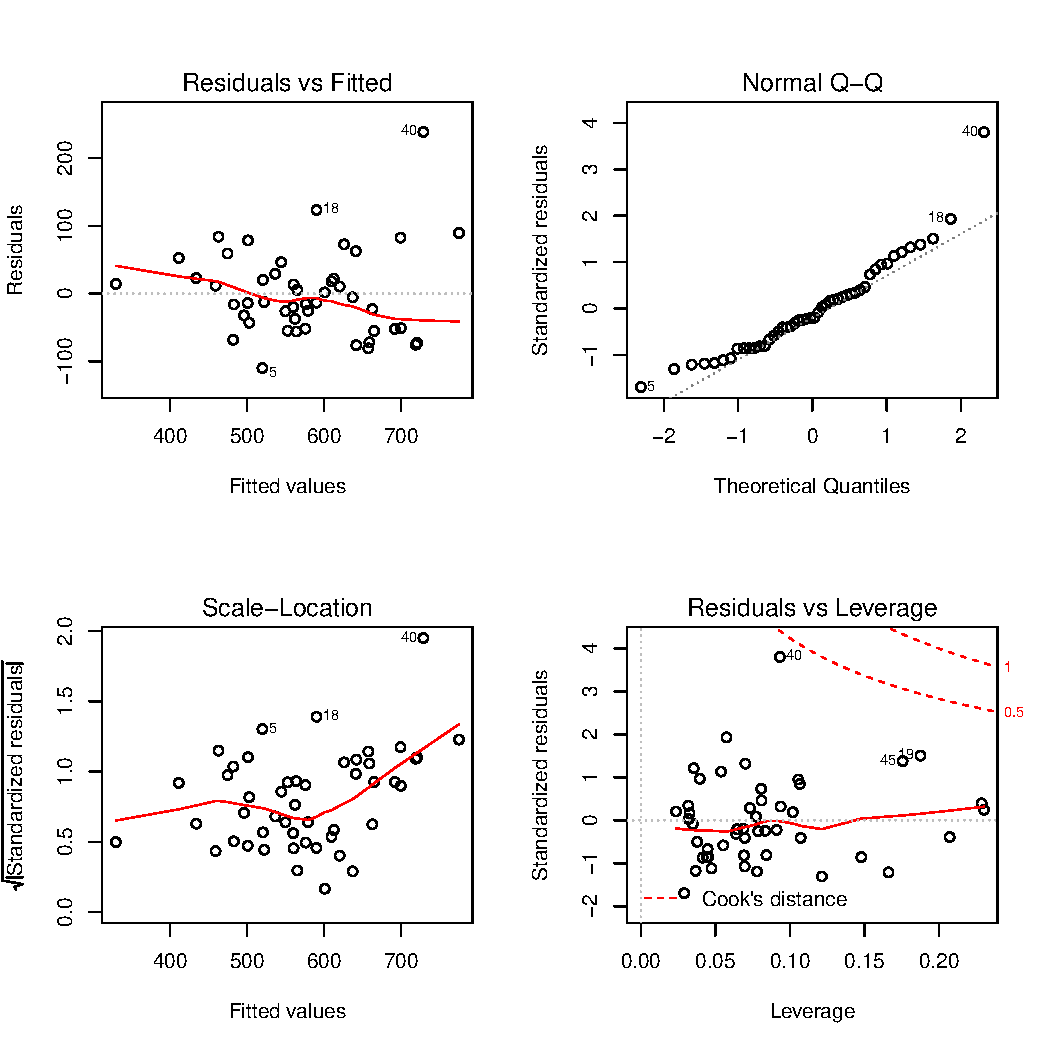
\includegraphics{P2-ML2_F_files/figure-latex/unnamed-chunk-6-1.pdf}

Se observa que la varianza no es constante, a medida que aumenta \(X\)
se observa que aumenta la varianza

A continuación presentamos el primer modelo propuesto :

\begin{Shaded}
\begin{Highlighting}[]
\NormalTok{Modelo1 <{-}}\StringTok{ }\KeywordTok{glm}\NormalTok{(y }\OperatorTok{\textasciitilde{}}\StringTok{ }\NormalTok{x, }\DataTypeTok{data=}\NormalTok{nueva\_data, }\DataTypeTok{family=}\KeywordTok{poisson}\NormalTok{(}\DataTypeTok{link =} \StringTok{"log"}\NormalTok{))}
\end{Highlighting}
\end{Shaded}

\begin{Shaded}
\begin{Highlighting}[]
\KeywordTok{summary}\NormalTok{(Modelo1)}
\end{Highlighting}
\end{Shaded}

\begin{verbatim}
## 
## Call:
## glm(formula = y ~ x, family = poisson(link = "log"), data = nueva_data)
## 
## Deviance Residuals: 
##       Min         1Q     Median         3Q        Max  
## -0.065468  -0.024434  -0.005905   0.012462   0.119165  
## 
## Coefficients:
##             Estimate Std. Error z value Pr(>|z|)
## (Intercept)  -6.9083     5.3907  -1.282    0.200
## x             0.2468     0.7967   0.310    0.757
## 
## (Dispersion parameter for poisson family taken to be 1)
## 
##     Null deviance: 0.26056  on 175  degrees of freedom
## Residual deviance: 0.16506  on 174  degrees of freedom
## AIC: Inf
## 
## Number of Fisher Scoring iterations: 8
\end{verbatim}

\begin{Shaded}
\begin{Highlighting}[]
\KeywordTok{exp}\NormalTok{(}\KeywordTok{coef}\NormalTok{(Modelo1))}
\end{Highlighting}
\end{Shaded}

\begin{verbatim}
##  (Intercept)            x 
## 0.0009994421 1.2798795770
\end{verbatim}

\textbf{Interpretación} \[\beta_0  estimado = -6.9083\]
\[\beta_1  estimado = 0.2468\]
\[\beta_0  estimado = exp(-6.9083)  \cong 0\]

Se espera que el número de reclamos por habitante de la región sea
aproximadamente cero cuando el logaritmo del número de accidentes de la
región es cero, es decir cuando el número de accidentes de la región es
uno.

\[\beta_1  estimado = exp(0.2468) \cong 1.28\]

Cuando ocurre un incremento de uno en el logaritmo del número de
accidentes de la región, se espera que esto genere un incremento de 29\%
en el número de reclamos por habitante de la región.

\textbf{b)} Realice gráficos de leverage, distancia de Cook, residuos
versus valores ajustados, residuos con bandas de confianza. Comente sus
resultados.

\textbf{Gráfico de Leverage y distancia de Cook}

\begin{Shaded}
\begin{Highlighting}[]
\KeywordTok{influenceIndexPlot}\NormalTok{(Modelo1,}\DataTypeTok{vars=}\KeywordTok{c}\NormalTok{ (}\StringTok{"Cook"}\NormalTok{, }\StringTok{"hat"}\NormalTok{), }\DataTypeTok{id=}\KeywordTok{list}\NormalTok{(}\DataTypeTok{n=}\DecValTok{5}\NormalTok{))}
\end{Highlighting}
\end{Shaded}

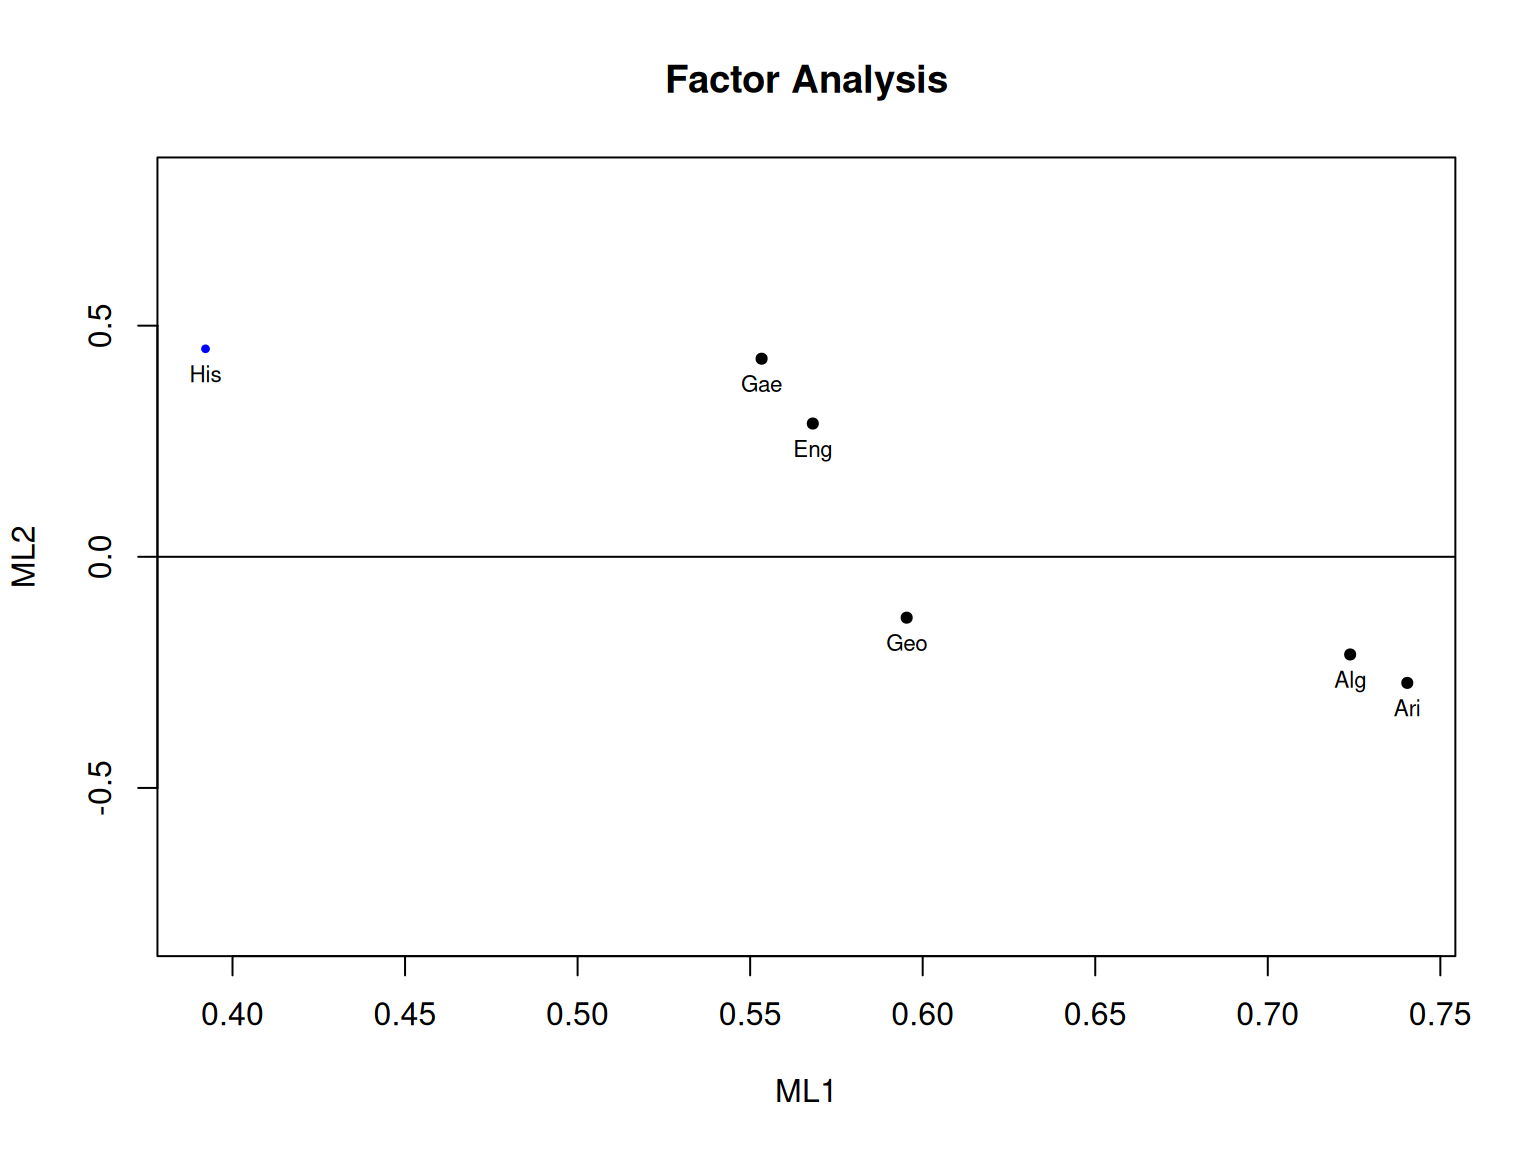
\includegraphics{P2-ML2_F_files/figure-latex/unnamed-chunk-9-1.pdf}

\textbf{Comentario} En el gráfico anterior de distancias de ``Cook D''
nos ayuda a identificar puntos que son potencialmente influyentes debido
a su ubicación en el rango de los datos.

También hay que notar el segundo gráfico donde se muestran los atípicos
en las covariables x, h(hatvalues). A esto se le conoce como leverage o
apalancamiento.

Se recomienda retirar los puntos con alta distancia de cook y alto
leverage effect(atípico en la covariable) como por ejemplo el punto 34.

\textbf{Gráfico de residuos versus valores ajustados}

\begin{Shaded}
\begin{Highlighting}[]
\KeywordTok{residualPlot}\NormalTok{(Modelo1,}\DataTypeTok{type=}\StringTok{"rstandard"}\NormalTok{)}
\end{Highlighting}
\end{Shaded}

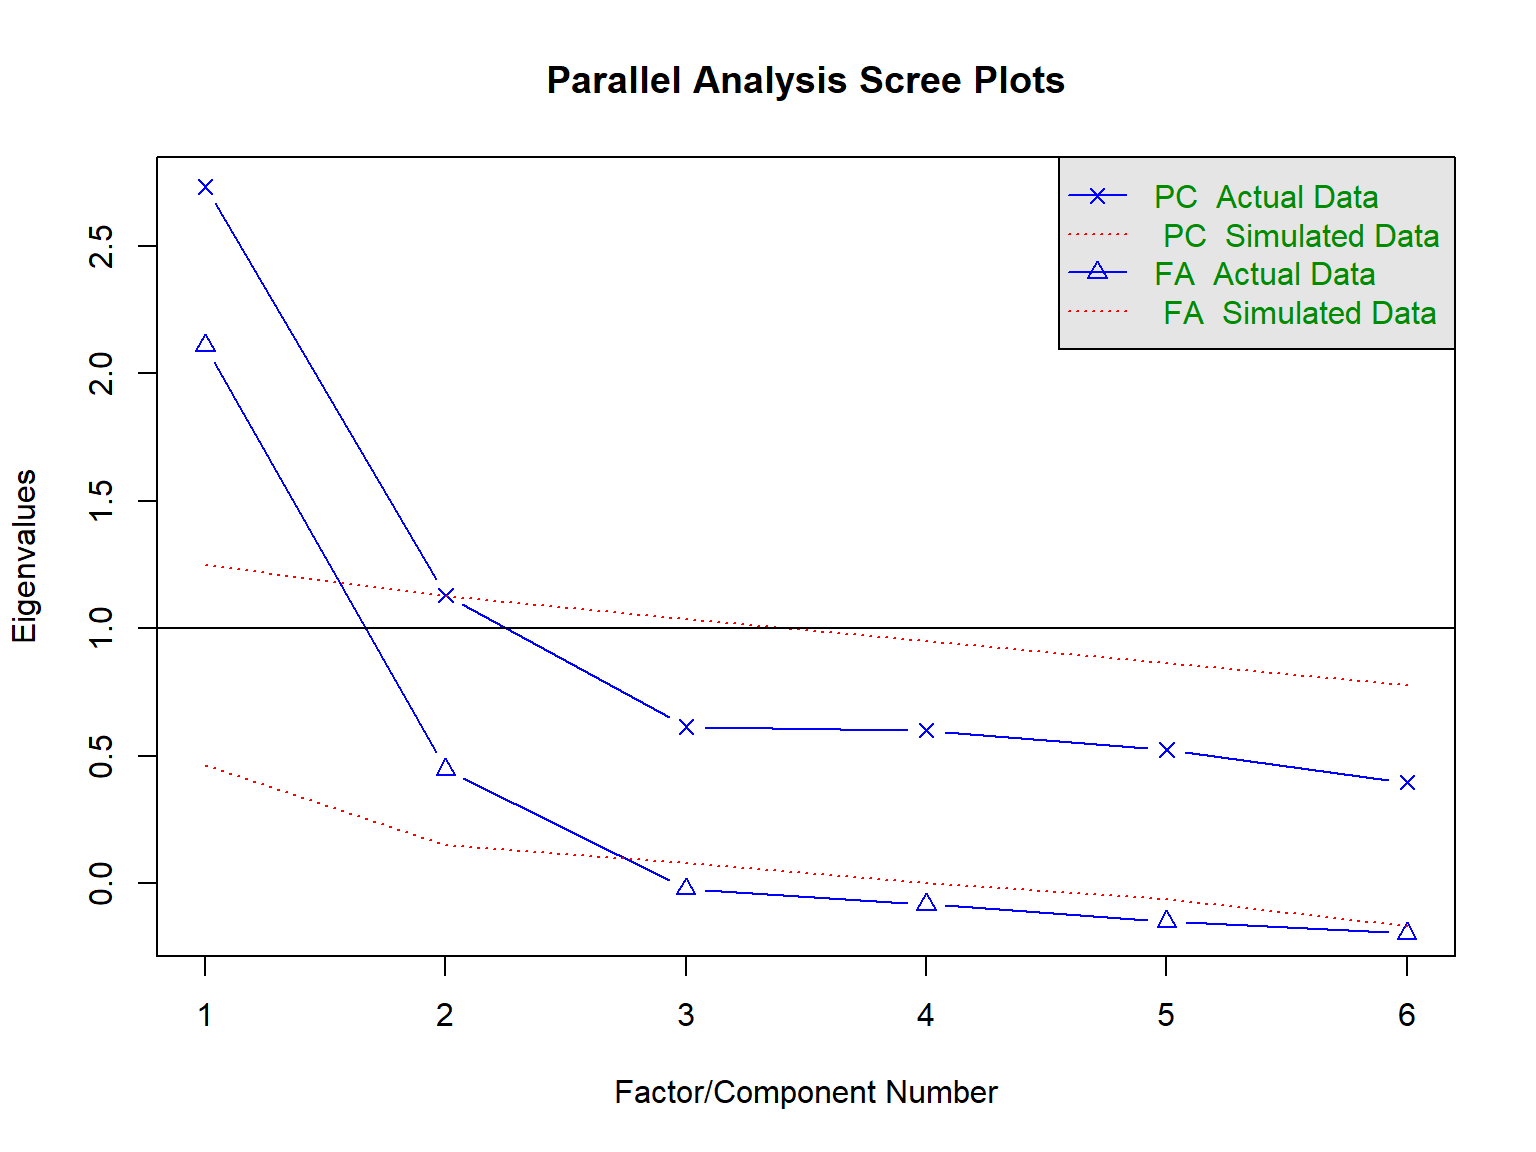
\includegraphics{P2-ML2_F_files/figure-latex/unnamed-chunk-10-1.pdf}

El modelo de Poisson es heterocedástico

Función de varianza: \[V(μ)=μ\]

No se muestra patrones, es casi casi un ruido blanco, pero parece que
hubiera mayor dispersión que en un modelo Poisson.

\textbf{Gráfico de residuos con bandas de confianza}

\begin{Shaded}
\begin{Highlighting}[]
\KeywordTok{library}\NormalTok{(hnp)}
\KeywordTok{hnp}\NormalTok{(Modelo1,}\DataTypeTok{halfnormal =} \OtherTok{FALSE}\NormalTok{)}
\end{Highlighting}
\end{Shaded}

\begin{verbatim}
## Poisson model
\end{verbatim}

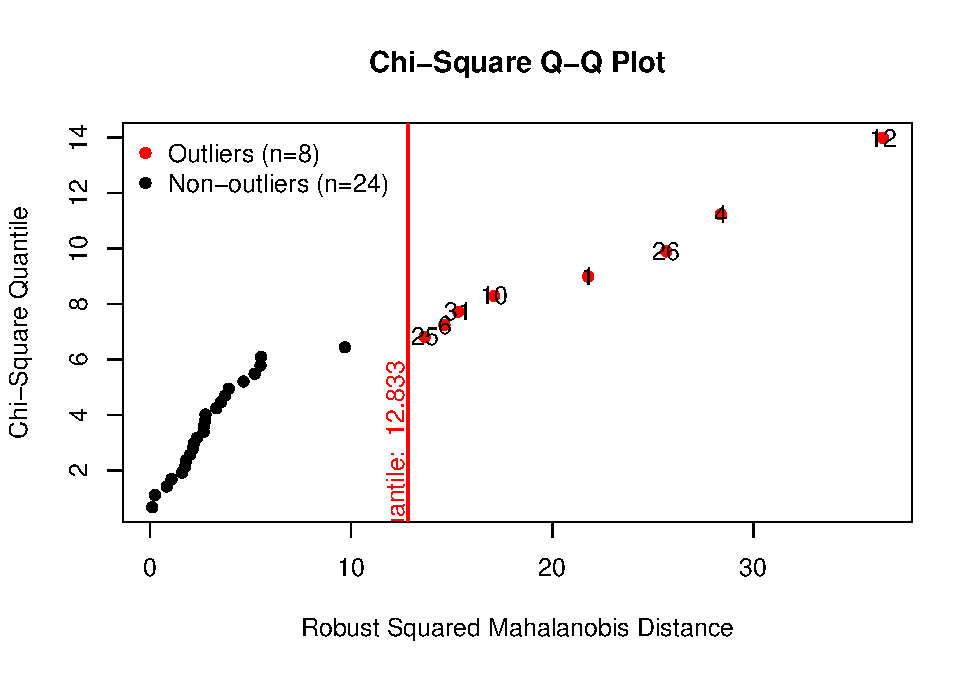
\includegraphics{P2-ML2_F_files/figure-latex/unnamed-chunk-11-1.pdf}

\textbf{Comentario }

Vemos que hay varios puntos que se quedan fuera de la banda, lo que
indica que este modelo no ajusta bien a los datos.

Este gráfico de bandas y el anterior de residuos, nos hace pensar que
necesitamos un modelo que contemple mayor varianza para que se ajuste
mejor a los datos, como el modelo Binomial Negativa.

\textbf{c)} En base a sus resultados en b) de ser necesario proponga un
nuevo modelo y realice un análisis de diagnóstico que incluya el estudio
del efecto de posibles observaciones infuyentes. Indique cuál sería el
modelo adecuado para este problema.

\textbf{Modelo 2 : Binomial Negativa}

\[Yi \sim BN(ui,\phi)\] \[n_i  = \beta_o + \beta_1 x_i\]
\[log(u_i)  = n_i\] \[E(Y_i)  = u_i\]
\[ Var(Y_i)  = u_i + \frac{u_i^2}{\phi}\] , tiene por propiedad más
varianza que el Modelo de Poisson.

Donde :

\begin{itemize}
\item
  \(Yi\) : número de reclamos por habitante de la región
\item
  \(Xi\) : logaritmo del número de accidentes en la región
\end{itemize}

Además, se retira del modelo el caso 34, por lo visto en los gráficos de
leverage y distancias de Cook.

\begin{Shaded}
\begin{Highlighting}[]
\NormalTok{Modelo2=}\KeywordTok{glm.nb}\NormalTok{(y }\OperatorTok{\textasciitilde{}}\StringTok{ }\NormalTok{x, }\DataTypeTok{data=}\NormalTok{nueva\_data, }\DataTypeTok{subset=}\OperatorTok{{-}}\DecValTok{34}\NormalTok{)}
\end{Highlighting}
\end{Shaded}

Coeficientes estimados

\begin{Shaded}
\begin{Highlighting}[]
\KeywordTok{summary}\NormalTok{(Modelo2)                  }
\end{Highlighting}
\end{Shaded}

\begin{verbatim}
## 
## Call:
## glm.nb(formula = y ~ x, data = nueva_data, subset = -34, init.theta = 70769.2186, 
##     link = log)
## 
## Deviance Residuals: 
##     Min       1Q   Median       3Q      Max  
## -0.2567  -0.1992  -0.1643   0.2433   0.3630  
## 
## Coefficients:
##             Estimate Std. Error z value Pr(>|z|)
## (Intercept)  -6.8135     5.4785  -1.244    0.214
## x             0.2307     0.8169   0.282    0.778
## 
## (Dispersion parameter for Negative Binomial(70769.22) family taken to be 1)
## 
##     Null deviance: 8.9247  on 174  degrees of freedom
## Residual deviance: 8.8453  on 173  degrees of freedom
## AIC: 15.56
## 
## Number of Fisher Scoring iterations: 1
## 
## 
##               Theta:  70769 
##           Std. Err.:  11219953 
## Warning while fitting theta: iteration limit reached 
## 
##  2 x log-likelihood:  -9.56
\end{verbatim}

\begin{Shaded}
\begin{Highlighting}[]
\KeywordTok{exp}\NormalTok{(}\KeywordTok{coef}\NormalTok{(Modelo2))}
\end{Highlighting}
\end{Shaded}

\begin{verbatim}
## (Intercept)           x 
## 0.001098867 1.259423018
\end{verbatim}

Gráfico de leverage y distancia de Cook

\begin{Shaded}
\begin{Highlighting}[]
\KeywordTok{influenceIndexPlot}\NormalTok{(Modelo2,}\DataTypeTok{vars=}\KeywordTok{c}\NormalTok{ (}\StringTok{"Cook"}\NormalTok{, }\StringTok{"hat"}\NormalTok{), }\DataTypeTok{id=}\KeywordTok{list}\NormalTok{(}\DataTypeTok{n=}\DecValTok{3}\NormalTok{))}
\end{Highlighting}
\end{Shaded}

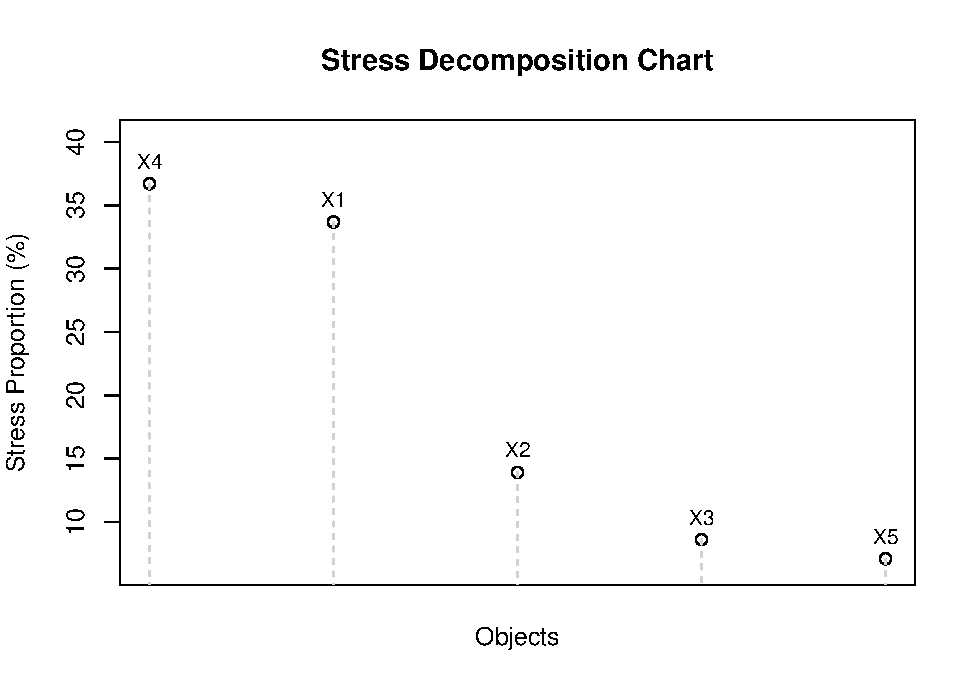
\includegraphics{P2-ML2_F_files/figure-latex/unnamed-chunk-14-1.pdf}

Del gráfico anterior , se recomienda retirar los puntos con alta
distancia de cook y alto leverage effect como por ejemplo el punto 13.

Gráfico de residuos versus valores ajustados

\begin{Shaded}
\begin{Highlighting}[]
\KeywordTok{residualPlot}\NormalTok{(Modelo2,}\DataTypeTok{type=}\StringTok{"rstandard"}\NormalTok{)}
\end{Highlighting}
\end{Shaded}

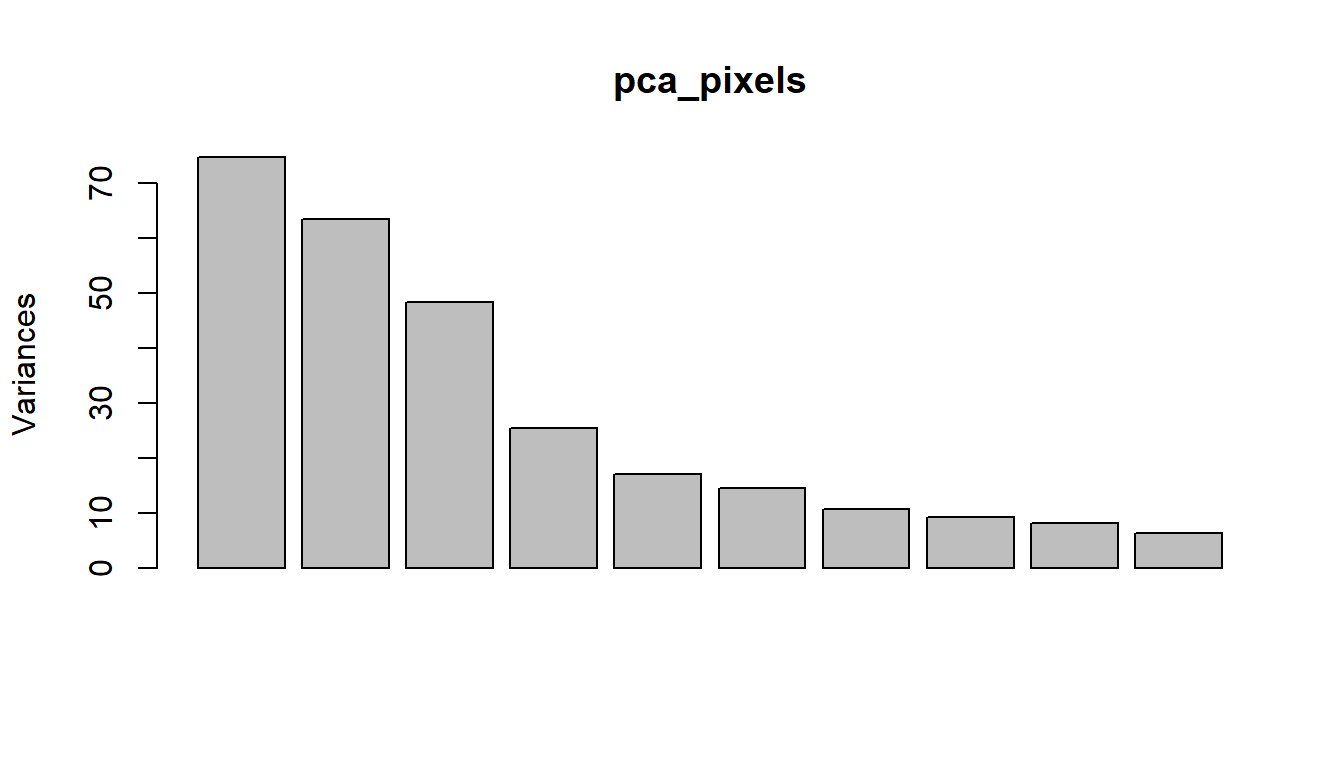
\includegraphics{P2-ML2_F_files/figure-latex/unnamed-chunk-15-1.pdf}

Gráfico de residuos con bandas de confianza

\begin{Shaded}
\begin{Highlighting}[]
\KeywordTok{hnp}\NormalTok{(Modelo2,}\DataTypeTok{halfnormal =} \OtherTok{FALSE}\NormalTok{)}
\end{Highlighting}
\end{Shaded}

\begin{verbatim}
## Negative binomial model (using MASS package)
\end{verbatim}

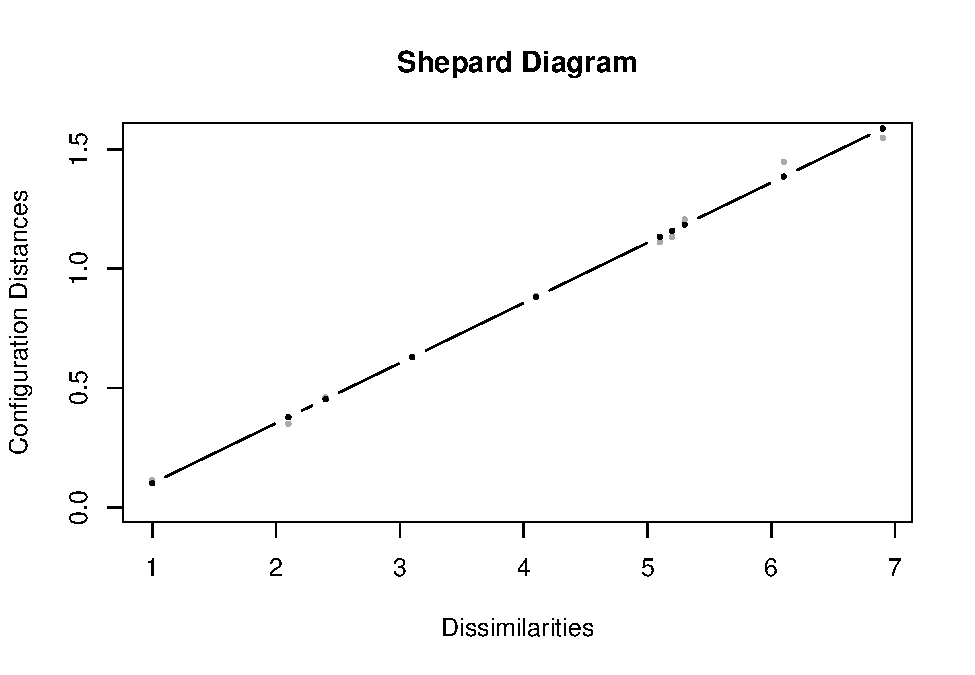
\includegraphics{P2-ML2_F_files/figure-latex/unnamed-chunk-16-1.pdf}

\textbf{Comentario} Vemos que los puntos están dentro de las bandas
hasta un punto donde se salen de las bandas y forman una región fuera de
ellas, lo que indica que este modelo tampoco ajusta bien a todos los
datos.

El gráfico de bandas de este modelo y del anterior nos hace pensar que
faltan considerar más covariables para encontrar un modelo que ajuste
mejor.

\textbf{d)} Si en una región hubiera un aumento del 10\% en el número de
accidentes, calcule en forma puntual y por intervalo el efecto en la
tasa de reclamos por habitante.

\textbf{Modelo 3 : Binomial Negativa}

\begin{Shaded}
\begin{Highlighting}[]
\NormalTok{Modelo3=}\KeywordTok{glm.nb}\NormalTok{(y }\OperatorTok{\textasciitilde{}}\StringTok{ }\NormalTok{x, }\DataTypeTok{data=}\NormalTok{nueva\_data, }\DataTypeTok{subset=}\OperatorTok{{-}}\KeywordTok{c}\NormalTok{(}\DecValTok{34}\NormalTok{,}\DecValTok{13}\NormalTok{))}
\end{Highlighting}
\end{Shaded}

Coeficientes estimados

\begin{Shaded}
\begin{Highlighting}[]
\KeywordTok{summary}\NormalTok{(Modelo3)                  }
\end{Highlighting}
\end{Shaded}

\begin{verbatim}
## 
## Call:
## glm.nb(formula = y ~ x, data = nueva_data, subset = -c(34, 13), 
##     init.theta = 71125.50582, link = log)
## 
## Deviance Residuals: 
##     Min       1Q   Median       3Q      Max  
## -0.2565  -0.1984  -0.1651   0.2434   0.3634  
## 
## Coefficients:
##             Estimate Std. Error z value Pr(>|z|)
## (Intercept)  -6.7600     5.5458  -1.219    0.223
## x             0.2214     0.8321   0.266    0.790
## 
## (Dispersion parameter for Negative Binomial(71125.51) family taken to be 1)
## 
##     Null deviance: 8.7910  on 173  degrees of freedom
## Residual deviance: 8.7206  on 172  degrees of freedom
## AIC: 15.423
## 
## Number of Fisher Scoring iterations: 1
## 
## 
##               Theta:  71126 
##           Std. Err.:  11404247 
## Warning while fitting theta: iteration limit reached 
## 
##  2 x log-likelihood:  -9.423
\end{verbatim}

\begin{Shaded}
\begin{Highlighting}[]
\KeywordTok{exp}\NormalTok{(}\KeywordTok{coef}\NormalTok{(Modelo3))}
\end{Highlighting}
\end{Shaded}

\begin{verbatim}
## (Intercept)           x 
## 0.001159269 1.247813474
\end{verbatim}

\[\beta_0  estimado = -6.7600\] \[\beta_1  estimado = 0.2214\]
\[\beta_0  estimado = exp(-6.7600)  \cong 0\]

Se espera que el número de reclamos por habitante de la región sea
aproximadamente cero cuando el logaritmo del número de accidentes de la
región es cero, es decir cuando el número de accidentes de la región es
uno.

\[\beta_1  estimado = exp(0.2214) \cong 1.25\]

Cuando ocurre un incremento de uno en el logaritmo del número de
accidentes de la región, se espera que esto genere un incremento de 25\%
en el número de reclamos por habitante de la región.

\textbf{Gráfico de Leverage y distancia de Cook}

\begin{Shaded}
\begin{Highlighting}[]
\KeywordTok{influenceIndexPlot}\NormalTok{(Modelo3,}\DataTypeTok{vars=}\KeywordTok{c}\NormalTok{ (}\StringTok{"Cook"}\NormalTok{, }\StringTok{"hat"}\NormalTok{), }\DataTypeTok{id=}\KeywordTok{list}\NormalTok{(}\DataTypeTok{n=}\DecValTok{3}\NormalTok{))}
\end{Highlighting}
\end{Shaded}

\includegraphics{P2-ML2_F_files/figure-latex/unnamed-chunk-19-1.pdf}

\textbf{Comentario} Se recomienda retirar los puntos con alta distancia
de cook y alto leverage effect(atípico en la covariable) , en este
modelo no tenemos puntos que cumplan ambas condiciones.

\textbf{Gráfico de residuos versus valores ajustados}

\begin{Shaded}
\begin{Highlighting}[]
\KeywordTok{residualPlot}\NormalTok{(Modelo3,}\DataTypeTok{type=}\StringTok{"rstandard"}\NormalTok{)}
\end{Highlighting}
\end{Shaded}

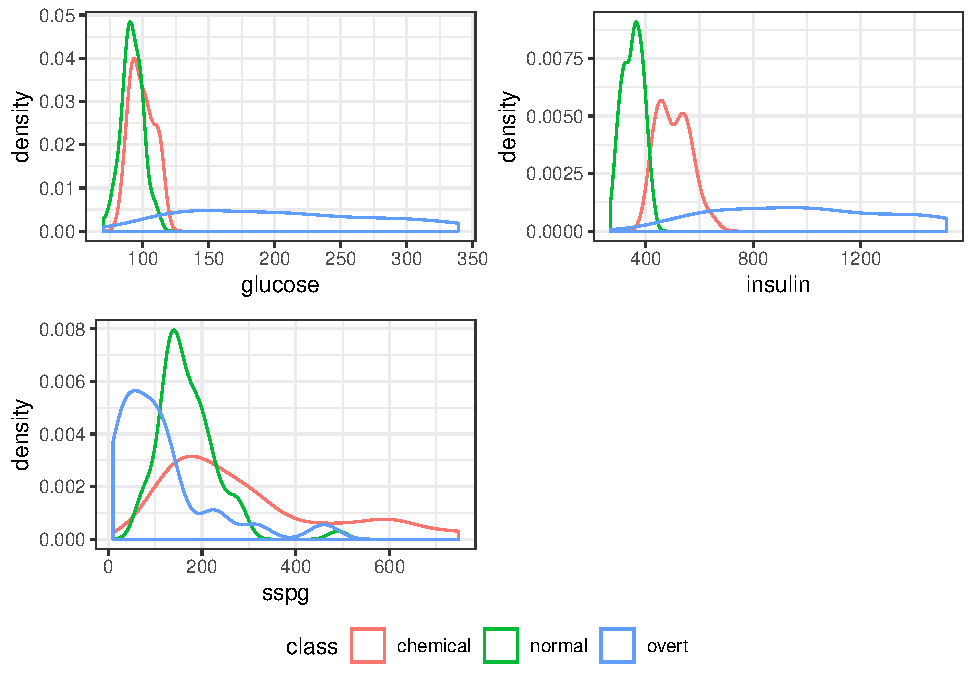
\includegraphics{P2-ML2_F_files/figure-latex/unnamed-chunk-20-1.pdf}

\textbf{Gráfico de residuos con bandas de confianza}

\begin{Shaded}
\begin{Highlighting}[]
\KeywordTok{hnp}\NormalTok{(Modelo3,}\DataTypeTok{halfnormal =} \OtherTok{FALSE}\NormalTok{)}
\end{Highlighting}
\end{Shaded}

\begin{verbatim}
## Negative binomial model (using MASS package)
\end{verbatim}

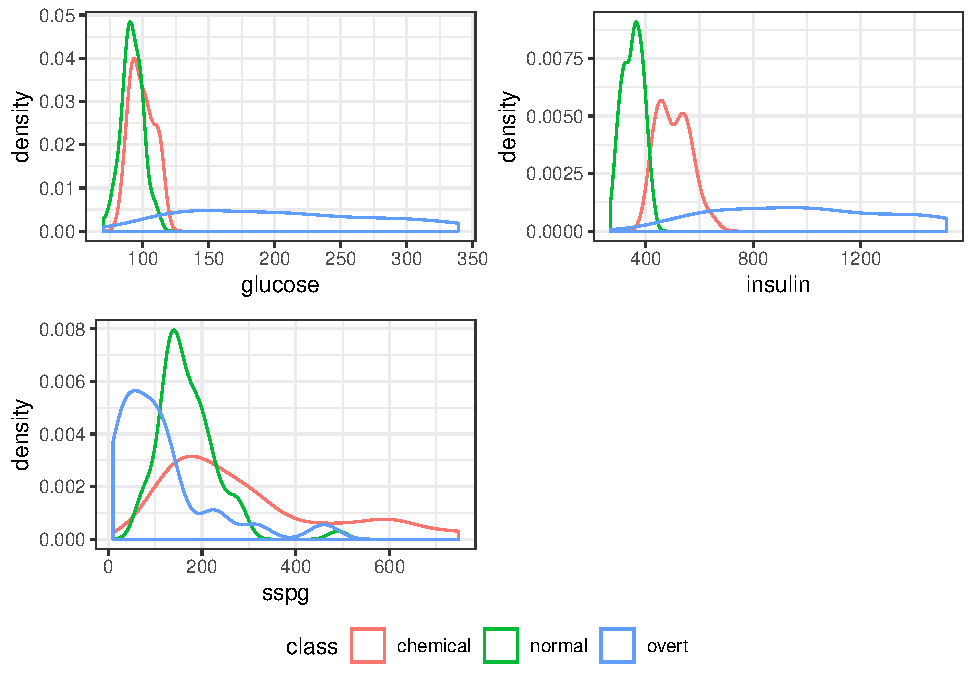
\includegraphics{P2-ML2_F_files/figure-latex/unnamed-chunk-21-1.pdf}

\begin{Shaded}
\begin{Highlighting}[]
\KeywordTok{AIC}\NormalTok{(Modelo1)}
\end{Highlighting}
\end{Shaded}

\begin{verbatim}
## [1] Inf
\end{verbatim}

\begin{Shaded}
\begin{Highlighting}[]
\KeywordTok{AIC}\NormalTok{(Modelo2)}
\end{Highlighting}
\end{Shaded}

\begin{verbatim}
## [1] 15.55971
\end{verbatim}

\begin{Shaded}
\begin{Highlighting}[]
\KeywordTok{AIC}\NormalTok{(Modelo3)}
\end{Highlighting}
\end{Shaded}

\begin{verbatim}
## [1] 15.42255
\end{verbatim}

Por el criterio AIC el mejor modelo es el \textbf{Modelo 3}

Pero el gráfico de bandas de residuos con bandas de confianza nos dice
que ninguno de estos 3 modelos ajusta bien a los datos, sugerimos
adicionar otras covariables que ayuden a explicar mejor.

\hypertarget{pregunta-4}{%
\subsection{Pregunta 4}\label{pregunta-4}}

La base de datos utilizada para el presente informe contiene las
siguientes variables:

\begin{itemize}
\tightlist
\item
  \textbf{Variable respuesta}

  \begin{itemize}
  \tightlist
  \item
    nsiniestros: Cantidad de siniestros ocurridos.
  \end{itemize}
\item
  \textbf{Covariables}

  \begin{itemize}
  \item
    Asegurados\_Total: Cantidad de asegurados en cada una de las
    pólizas.
  \item
    Planilla\_total: Monto mensual de salario pagado a los empleados en
    unidades monetarias dentro de cada póliza.
  \item
    nivel\_riesgo: Esta variable fue construida clasificando las
    actividades de riesgo del 1 al 5, donde 5 significa que la actividad
    económica que desarrolla la empresa tiene mayor exposición al riesgo
    de accidente o enfermedad profesional y 1 que la exposición a estos
    riesgos es menor.
  \end{itemize}
\end{itemize}

La presente base de datos contiene 14,064 observaciones. Estas
observaciones fueron recabadas por un período de 3 años.

\textbf{Objetivo}

El objetivo de este análisis es modelar el número de reclamos de una
póliza de seguro de vida contratada para un grupo asegurado (que
consiste en todos los empleados de una empresa), mediante las variables
explicativas: número de asegurados, planilla mensual (salario mensual
del grupo) y nivel de riesgo de la actividad económica de la empresa.

Los datos considerados en el análisis contemplan las Pólizas vigentes a
corte dic/2017 de un producto de Seguro de Vida de una Compañía de
Seguros de Perú. En cada una de estas pólizas al menos uno de los
miembros del grupo asegurado ha presentado un reclamo de invalidez o los
familiares de los miembros del grupo han presentado por lo menos un
reclamo de fallecimiento en un periodo de tres años.

El estudio se compone de un análisis exploratorio de los datos,
selección del mejor modelo, análisis de diagnóstico del mismo e
interpretación de resultados.

\hypertarget{anuxe1lisis-exploratorio}{%
\subsubsection{Análisis Exploratorio}\label{anuxe1lisis-exploratorio}}

Para realizar el análisis exploratorio inicial, realizaremos la carga de
los datos en el siguiente código:

\begin{Shaded}
\begin{Highlighting}[]
\KeywordTok{library}\NormalTok{(dplyr)}
\KeywordTok{library}\NormalTok{(car)}
\KeywordTok{library}\NormalTok{(ggplot2)}
\KeywordTok{library}\NormalTok{(car)}
\KeywordTok{library}\NormalTok{(GGally)}
\KeywordTok{library}\NormalTok{(stargazer)}
\KeywordTok{library}\NormalTok{(hnp)}
\KeywordTok{setwd}\NormalTok{(}\StringTok{"/home/justomanrique/Documents/maestria{-}pucp/2019{-}2/modelos{-}lineales{-}2/clase{-}7/"}\NormalTok{)}
\NormalTok{datos\_preg4 <{-}}\StringTok{ }\NormalTok{readxl}\OperatorTok{::}\KeywordTok{read\_excel}\NormalTok{(}\StringTok{"pregunta4\_diana\_v2.xlsx"}\NormalTok{)}

\NormalTok{datos\_preg4 =}\StringTok{ }\NormalTok{datos\_preg4 }\OperatorTok{\%>\%}
\StringTok{  }\KeywordTok{mutate}\NormalTok{ (  }\DataTypeTok{ACTIVIDAd=}\KeywordTok{as.factor}\NormalTok{(ACTIVIDAd),}
            \DataTypeTok{nivel\_riesgo=}\KeywordTok{as.factor}\NormalTok{(nivel\_riesgo))}
\end{Highlighting}
\end{Shaded}

Realizamos un gráfico de dispersión mediante la función ggpairs, para
identificar posibles relaciones entre los datos así como la distribución
de las mismas:

\begin{Shaded}
\begin{Highlighting}[]
\NormalTok{nombres =}\StringTok{ }\KeywordTok{c}\NormalTok{(}\StringTok{"ACTIVIDAd"}\NormalTok{,}\StringTok{"Asegurados\_total"}\NormalTok{,}\StringTok{"Planilla\_total"}\NormalTok{,}\StringTok{"nsiniestros"}\NormalTok{,}\StringTok{"nivel\_riesgo"}\NormalTok{)}
\NormalTok{datos\_preg4 =}\StringTok{ }\KeywordTok{subset}\NormalTok{ ( datos\_preg4 , }\DataTypeTok{select =}\NormalTok{ nombres )}
\NormalTok{datos\_preg4 =}\StringTok{ }\KeywordTok{na.omit}\NormalTok{ ( datos\_preg4 )}

\NormalTok{datos\_preg4 =}\StringTok{ }\NormalTok{datos\_preg4 }\OperatorTok{\%>\%}
\StringTok{  }\KeywordTok{mutate}\NormalTok{ (  }\DataTypeTok{ACTIVIDAd=}\KeywordTok{as.factor}\NormalTok{(ACTIVIDAd),}
            \DataTypeTok{nivel\_riesgo=}\KeywordTok{as.factor}\NormalTok{(nivel\_riesgo))}

\NormalTok{datos\_preg4 =}\StringTok{ }\NormalTok{datos\_preg4[,}\DecValTok{2}\OperatorTok{:}\DecValTok{5}\NormalTok{]}

\KeywordTok{summary}\NormalTok{(datos\_preg4)}
\end{Highlighting}
\end{Shaded}

\begin{verbatim}
##  Asegurados_total   Planilla_total      nsiniestros       nivel_riesgo
##  Min.   :    1.00   Min.   :       2   Min.   : 0.00000   1:1063      
##  1st Qu.:    6.00   1st Qu.:    8075   1st Qu.: 0.00000   2:1736      
##  Median :   11.00   Median :   14300   Median : 0.00000   3:1183      
##  Mean   :   37.26   Mean   :   76161   Mean   : 0.01465   4:5705      
##  3rd Qu.:   25.00   3rd Qu.:   36496   3rd Qu.: 0.00000   5:4377      
##  Max.   :13401.00   Max.   :50044818   Max.   :24.00000
\end{verbatim}

En base a ello se observa:

\begin{itemize}
\tightlist
\item
  La cartera de pólizas en el presente informe es riesgosa, pues existe
  mayor proporción de pólizas con riesgo 4 y 5 que de pólizas con riesgo
  1 a 3.
\item
  En las variables Asegurados\_total, Planilla\_total, nsiniestros
  existen valores extremos pues la gráfica se encuentra distorsionada,
  con alta concentración de valores en un lado y una cola larga hacia la
  derecha.
\item
  Se observa correlación fuerte entre la cantidad total de asegurados y
  planilla (correlación del 0.736).
\item
  Se observa correlación media entre la cantidad de siniestros y la
  planilla total (correlación del 0.513).
\end{itemize}

\hypertarget{selecciuxf3n-de-modelos}{%
\subsubsection{Selección de modelos}\label{selecciuxf3n-de-modelos}}

\begin{Shaded}
\begin{Highlighting}[]
\NormalTok{modelo1 <{-}}\StringTok{ }\KeywordTok{glm}\NormalTok{(nsiniestros }\OperatorTok{\textasciitilde{}}\StringTok{ }\KeywordTok{log}\NormalTok{(Asegurados\_total) }\OperatorTok{+}\StringTok{ }\KeywordTok{log}\NormalTok{(Planilla\_total) }\OperatorTok{+}\StringTok{ }\NormalTok{nivel\_riesgo, }
\DataTypeTok{data=}\NormalTok{datos\_preg4, }\DataTypeTok{family=}\KeywordTok{poisson}\NormalTok{(}\DataTypeTok{link =} \StringTok{"log"}\NormalTok{))}

\KeywordTok{summary}\NormalTok{(modelo1)}
\end{Highlighting}
\end{Shaded}

\begin{verbatim}
## 
## Call:
## glm(formula = nsiniestros ~ log(Asegurados_total) + log(Planilla_total) + 
##     nivel_riesgo, family = poisson(link = "log"), data = datos_preg4)
## 
## Deviance Residuals: 
##     Min       1Q   Median       3Q      Max  
## -3.9422  -0.1022  -0.0617  -0.0429  13.1714  
## 
## Coefficients:
##                        Estimate Std. Error z value Pr(>|z|)    
## (Intercept)           -17.78446    0.81749 -21.755  < 2e-16 ***
## log(Asegurados_total)   0.07980    0.11724   0.681  0.49608    
## log(Planilla_total)     1.04650    0.09911  10.559  < 2e-16 ***
## nivel_riesgo2           0.65363    0.40554   1.612  0.10702    
## nivel_riesgo3           1.42285    0.43321   3.284  0.00102 ** 
## nivel_riesgo4           1.30232    0.31807   4.094 4.23e-05 ***
## nivel_riesgo5           1.71826    0.32990   5.208 1.90e-07 ***
## ---
## Signif. codes:  0 '***' 0.001 '**' 0.01 '*' 0.05 '.' 0.1 ' ' 1
## 
## (Dispersion parameter for poisson family taken to be 1)
## 
##     Null deviance: 2267.5  on 14063  degrees of freedom
## Residual deviance: 1163.7  on 14057  degrees of freedom
## AIC: 1413.9
## 
## Number of Fisher Scoring iterations: 8
\end{verbatim}

\begin{Shaded}
\begin{Highlighting}[]
\KeywordTok{round}\NormalTok{(}\KeywordTok{exp}\NormalTok{(}\KeywordTok{coef}\NormalTok{(modelo1)),}\DecValTok{3}\NormalTok{)}
\end{Highlighting}
\end{Shaded}

\begin{verbatim}
##           (Intercept) log(Asegurados_total)   log(Planilla_total) 
##                 0.000                 1.083                 2.848 
##         nivel_riesgo2         nivel_riesgo3         nivel_riesgo4 
##                 1.923                 4.149                 3.678 
##         nivel_riesgo5 
##                 5.575
\end{verbatim}

Del modelo inicial, se puede observar que:

\begin{itemize}
\tightlist
\item
  En la medida que incremente el nivel de riesgo (tomando como
  referencia el nivel 1), se espera un incremento en la cantidad de
  siniestros. El efecto se hace mayor, en la medida que el nivel de
  riesgo incrementa (ver tabla de coeficientes).
\item
  En la medida que incremente la cantidad de asegurados, se espera que
  incremente el 8\% la cantidad de siniestros.
\item
  En la medida que aumente la planilla total, se espera que se
  incremente en 180\% la cantidad de siniestros.
\end{itemize}

\hypertarget{anuxe1lisis-de-diagnuxf3stico}{%
\subsubsection{Análisis de
diagnóstico}\label{anuxe1lisis-de-diagnuxf3stico}}

La interpretación anteriormente indicada se sostiene en la medida que
los supuestos del modelo se cumplan. Para ello, se realizó el siguiente
análisis de diagnóstico:

\hypertarget{residuales}{%
\paragraph{Residuales}\label{residuales}}

Ver a continuación el diagnóstico de residuales:

\begin{Shaded}
\begin{Highlighting}[]
\CommentTok{\#\#\#Gráfico de residuos con bandas de confianza}
\KeywordTok{hnp}\NormalTok{(modelo1,}\DataTypeTok{halfnormal =} \OtherTok{FALSE}\NormalTok{)}
\end{Highlighting}
\end{Shaded}

\begin{verbatim}
## Poisson model
\end{verbatim}

\includegraphics{P2-ML2_F_files/figure-latex/residuales-1.pdf}

Se observa, en el diagnóstico de residuales, que los residuos se ajustan
adecuadamente a las bandas de confianza. Sin embargo, en las colas
existe mayor dispersión. Esto podría deberse a los valores atípicos que
existen dentro de la muestra (esto se observó en el análisis
exploratorio).

\hypertarget{visualizaciuxf3n-de-puntos-influyentes}{%
\paragraph{Visualización de puntos
influyentes}\label{visualizaciuxf3n-de-puntos-influyentes}}

\begin{Shaded}
\begin{Highlighting}[]
\CommentTok{\#\#\#Gráfico de leverage y distancia de Cook}
\KeywordTok{influenceIndexPlot}\NormalTok{(modelo1,}\DataTypeTok{vars=}\KeywordTok{c}\NormalTok{ (}\StringTok{"Cook"}\NormalTok{, }\StringTok{"hat"}\NormalTok{), }\DataTypeTok{id=}\KeywordTok{list}\NormalTok{(}\DataTypeTok{n=}\DecValTok{3}\NormalTok{))}
\end{Highlighting}
\end{Shaded}

\includegraphics{P2-ML2_F_files/figure-latex/puntos influyentes-1.pdf}

Se observa que las observaciones 1296,457 y 2274 son valores influyentes
en el modelo de acuerdo a la distancia de Cook. Asimismo, en relación a
los hat-values, las observaciones 47, 1296 y 12627 son valores
influyentes.

\hypertarget{modelo-final}{%
\subsubsection{Modelo final}\label{modelo-final}}

En base al trabajo anterior, se eliminaron los valores influyentes en
común para evaluar el modelo final. Ver a continuación

\begin{Shaded}
\begin{Highlighting}[]
\CommentTok{\# Modelo 2: Poisson Regression y \textasciitilde{} x {-}c(1296,47)}
\NormalTok{modelo2 <{-}}\StringTok{ }\KeywordTok{glm}\NormalTok{(nsiniestros }\OperatorTok{\textasciitilde{}}\StringTok{ }\KeywordTok{log}\NormalTok{(Asegurados\_total) }\OperatorTok{+}\StringTok{ }\KeywordTok{log}\NormalTok{(Planilla\_total) }\OperatorTok{+}\StringTok{ }\NormalTok{nivel\_riesgo, }\DataTypeTok{data=}\NormalTok{datos\_preg4, }\DataTypeTok{family=}\KeywordTok{poisson}\NormalTok{(}\DataTypeTok{link =} \StringTok{"log"}\NormalTok{), }\DataTypeTok{subset =} \OperatorTok{{-}}\KeywordTok{c}\NormalTok{(}\DecValTok{1296}\NormalTok{,}\DecValTok{47}\NormalTok{))}

\KeywordTok{summary}\NormalTok{(modelo2)}
\end{Highlighting}
\end{Shaded}

\begin{verbatim}
## 
## Call:
## glm(formula = nsiniestros ~ log(Asegurados_total) + log(Planilla_total) + 
##     nivel_riesgo, family = poisson(link = "log"), data = datos_preg4, 
##     subset = -c(1296, 47))
## 
## Deviance Residuals: 
##     Min       1Q   Median       3Q      Max  
## -2.9718  -0.1027  -0.0620  -0.0425  13.0147  
## 
## Coefficients:
##                       Estimate Std. Error z value Pr(>|z|)    
## (Intercept)           -16.5470     0.9316 -17.761  < 2e-16 ***
## log(Asegurados_total)   0.2977     0.1307   2.279  0.02268 *  
## log(Planilla_total)     0.8625     0.1132   7.620 2.53e-14 ***
## nivel_riesgo2           0.6561     0.4062   1.615  0.10628    
## nivel_riesgo3           1.4274     0.4354   3.278  0.00105 ** 
## nivel_riesgo4           1.3058     0.3234   4.038 5.39e-05 ***
## nivel_riesgo5           1.7427     0.3315   5.257 1.47e-07 ***
## ---
## Signif. codes:  0 '***' 0.001 '**' 0.01 '*' 0.05 '.' 0.1 ' ' 1
## 
## (Dispersion parameter for poisson family taken to be 1)
## 
##     Null deviance: 1972.2  on 14061  degrees of freedom
## Residual deviance: 1142.3  on 14055  degrees of freedom
## AIC: 1387.4
## 
## Number of Fisher Scoring iterations: 8
\end{verbatim}

\begin{Shaded}
\begin{Highlighting}[]
\CommentTok{\#ha cambiado la estimacion de los parametros beta y el log(asegurados\_total se ha vuelto significativo)}

\KeywordTok{round}\NormalTok{(}\KeywordTok{exp}\NormalTok{(}\KeywordTok{coef}\NormalTok{(modelo2)),}\DecValTok{3}\NormalTok{)}
\end{Highlighting}
\end{Shaded}

\begin{verbatim}
##           (Intercept) log(Asegurados_total)   log(Planilla_total) 
##                 0.000                 1.347                 2.369 
##         nivel_riesgo2         nivel_riesgo3         nivel_riesgo4 
##                 1.927                 4.168                 3.691 
##         nivel_riesgo5 
##                 5.713
\end{verbatim}

Se observa que la estimación de los parámetros ha variado
considerablemente para la cantidad total de asegurados (1.347
vs.~1.083), así como para la planilla (2.369 vs.~2.848). Asimismo, se
observa que la cantidad total de asegurados se ha vuelto una variable
significativa.

Asimismo, se han hecho los siguientes diagnósticos.

\begin{Shaded}
\begin{Highlighting}[]
\CommentTok{\#\#\#\#\#\#\#\#\#\#\#\#\#\#}
\CommentTok{\#\#\#Grafico de leverage y distancia de Cook}

\KeywordTok{influenceIndexPlot}\NormalTok{(modelo2,}\DataTypeTok{vars=}\KeywordTok{c}\NormalTok{ (}\StringTok{"Cook"}\NormalTok{, }\StringTok{"hat"}\NormalTok{), }\DataTypeTok{id=}\KeywordTok{list}\NormalTok{(}\DataTypeTok{n=}\DecValTok{3}\NormalTok{))}
\end{Highlighting}
\end{Shaded}

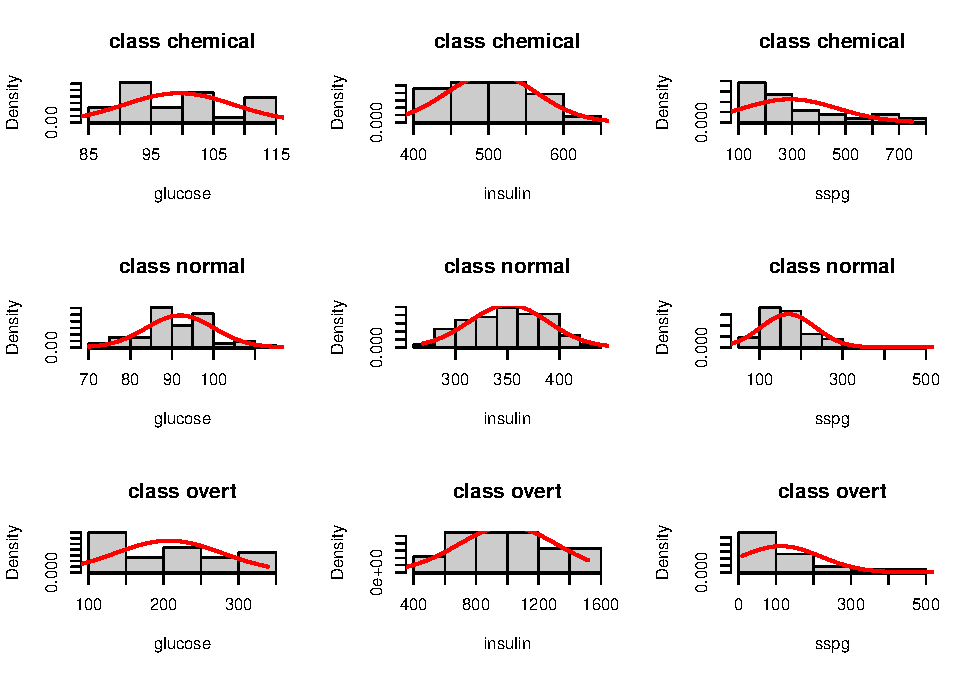
\includegraphics{P2-ML2_F_files/figure-latex/unnamed-chunk-25-1.pdf}

\begin{Shaded}
\begin{Highlighting}[]
\CommentTok{\#\#\#Gr?fico de residuos versus valores ajustados}
\KeywordTok{residualPlot}\NormalTok{(modelo2,}\DataTypeTok{type=}\StringTok{"rstandard"}\NormalTok{)}
\end{Highlighting}
\end{Shaded}

\includegraphics{P2-ML2_F_files/figure-latex/unnamed-chunk-25-2.pdf}

\begin{Shaded}
\begin{Highlighting}[]
\CommentTok{\#\#\#Gr?fico de residuos con bandas de confianza}
\KeywordTok{hnp}\NormalTok{(modelo2,}\DataTypeTok{halfnormal =} \OtherTok{FALSE}\NormalTok{)}
\end{Highlighting}
\end{Shaded}

\begin{verbatim}
## Poisson model
\end{verbatim}

\includegraphics{P2-ML2_F_files/figure-latex/unnamed-chunk-25-3.pdf}

En relación a los gráficos presentados, se visualiza lo siguiente:

\begin{itemize}
\tightlist
\item
  Se observa que los residuales se encuentran más cerca a las bandas de
  confianza de los residuales, sin embargo aún persisten ciertos valores
  influyentes.
\item
  Se observa que aún siguen persistiendo valores influyentes.
\end{itemize}


\end{document}
